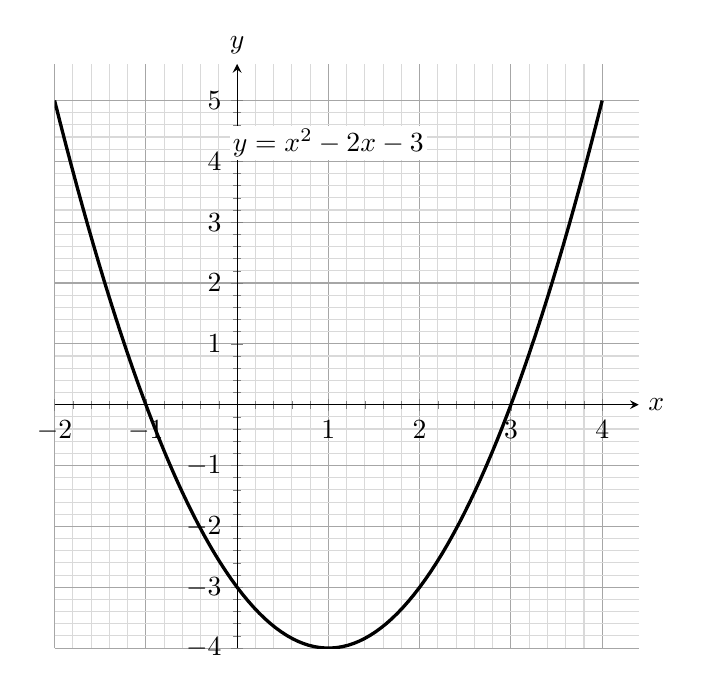
\begin{tikzpicture}
  \begin{axis}[
    width=9cm, height=9cm,
    axis lines=middle, xlabel={$x$}, ylabel={$y$},
    xmin=-2, xmax=4.4, ymin=-4, ymax=5.6,
    xtick={-2,...,4}, ytick={-4,...,5},
    minor x tick num=4, minor y tick num=4,
    grid=both, major grid style={gray!70}, minor grid style={gray!30},
    every axis x label/.style={at={(ticklabel* cs:1.0)}, anchor=west},
    every axis y label/.style={at={(ticklabel* cs:1.0)}, anchor=south},
  ]
    \addplot[very thick, domain=-2:4, samples=100] {x^2 - 2*x - 3};
    \node[fill=white, inner sep=1pt] at (axis cs:1,4.3) {$y = x^2 - 2x - 3$};
  \end{axis}
\end{tikzpicture}
